% !TeX root = main.tex
\chapter{Operational Evidence}
\label{appendix:observability_submit_ui}
\label{appendix:submit_service_ui}

This appendix records the evidence and browser-side inspection surfaces that support the implementation and evaluation chapters. The main implementation chapter focuses on the execution path; the details here explain how run state, metrics, artefacts, logs, and UI views are retained for inspection and repeatable execution.

\section{Physical Testbed}
\label{appendix:physical_testbed}

Figure~\ref{fig:cluster_physical_worker_pool} shows the physical worker pool behind the experiments. The evaluation uses logical deployment slices from this shared hardware rather than all visible devices in every run.

\begin{figure}[H]
\centering
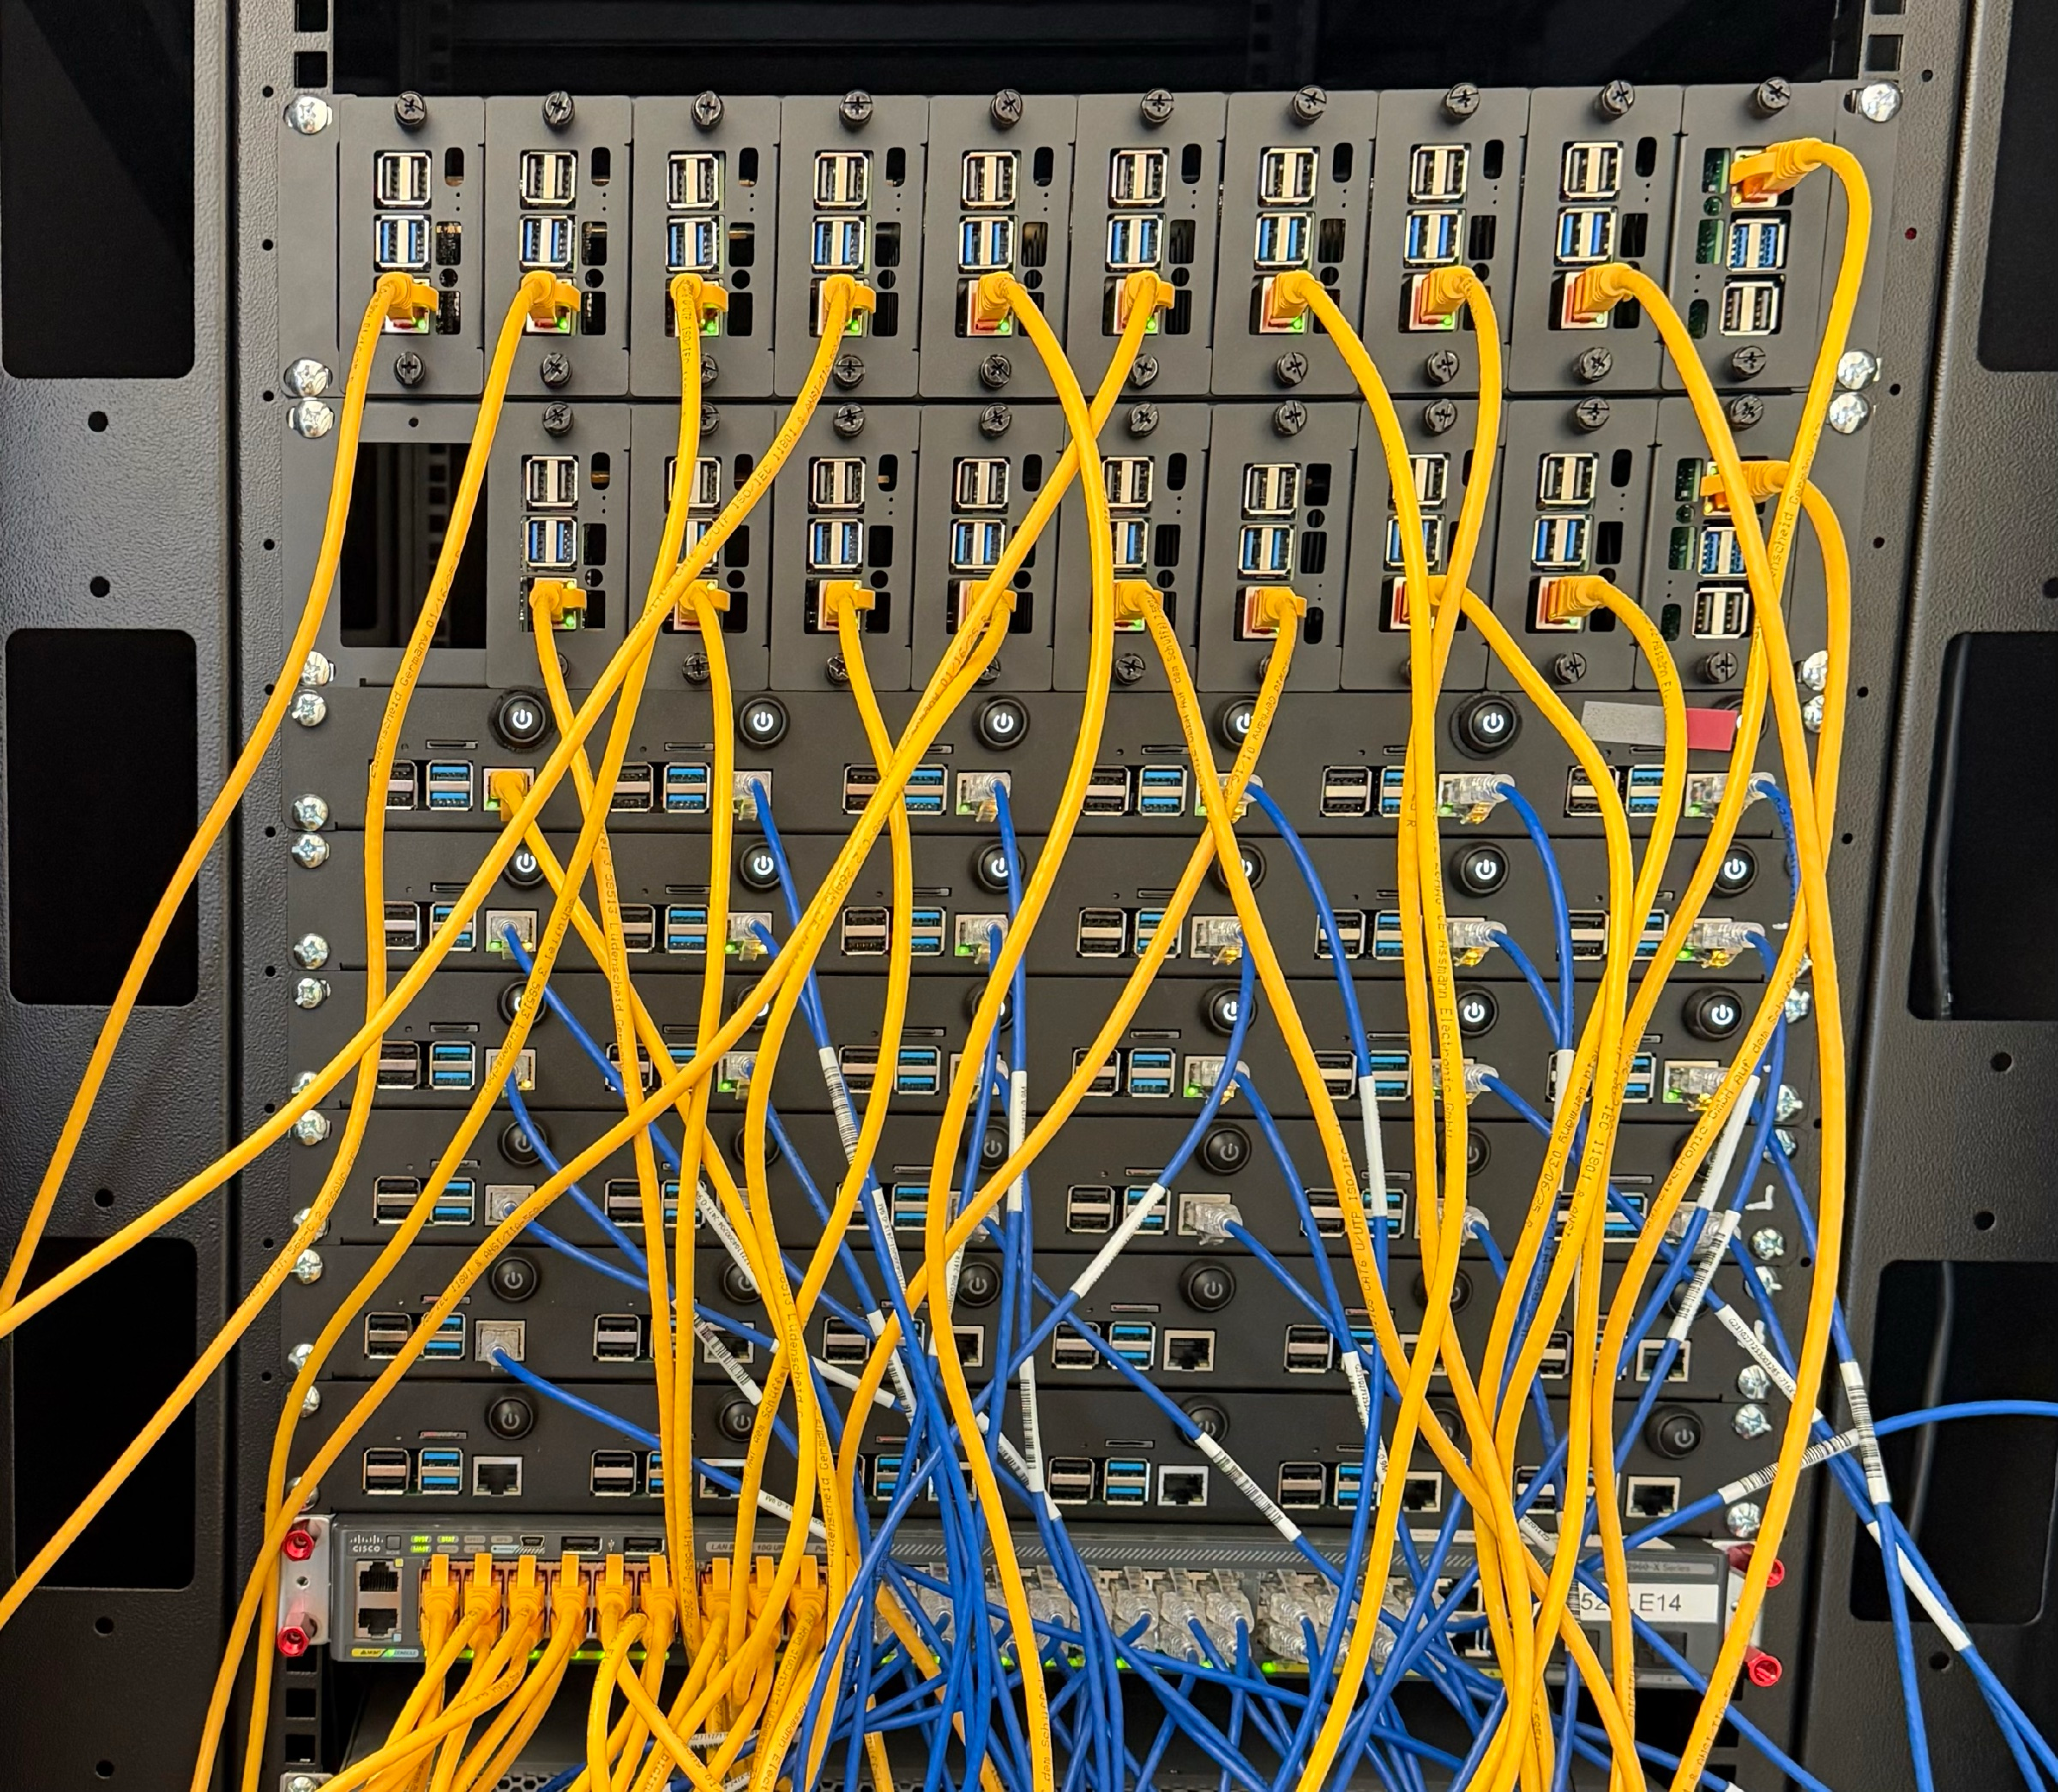
\includegraphics[width=0.72\textwidth]{figures/clusterpicture.pdf}
\caption{\textbf{Physical Raspberry Pi worker pool used for the experiments.} The cluster provides the mixed \texttt{rpi4}/\texttt{rpi5} substrate used by \texttt{fedctl}; individual experiments select logical deployment slices from this shared hardware.}
\label{fig:cluster_physical_worker_pool}
\end{figure}

\section{Observability and Reproducibility}
\label{appendix:observability_reproducibility}

The observability layer is organised around the questions that the evaluation and operator need to answer.

\paragraph{Did the run finish, and with which config/image?}
The submit service records submission identity, runner arguments, reconstructed command, status, errors, and result location. W\&B records method, task, profile tag, submission ID, and attempt metadata. Together these fields provide operational and scientific provenance.

\paragraph{Which physical devices participated?}
Nomad placement metadata and client-app environment variables are propagated into client logs and metrics. The research app records device type, node identity where available, partition ID, model rate, and typed-partition metadata.

\paragraph{How long did local training and evaluation take?}
Client replies include training duration, evaluation duration, examples per second, number of examples, and model rate. These metrics support the compute timing diagnostics in Table~\ref{tab:compute_main_runtime} and Figure~\ref{fig:compute_cifar10_client_train_time}.

\paragraph{Did asynchronous methods underrepresent \texttt{rpi4} clients?}
The asynchronous loop logs accepted updates with device type, staleness, queue latency, training duration, client trip, server step, and applied weight. These outputs support the participation, staleness, and weight-share analyses in Figures~\ref{fig:network_async_participation_staleness}--\ref{fig:network_async_weight_violin}.

\paragraph{Which artefacts regenerate the tables and figures?}
W\&B histories and summaries provide curves, final scores, runtime, target status, and fairness summaries. Structured artefacts provide event-level and per-client rows; submit-service log archives provide operational evidence for debugging and repeatable execution.

\section{Submit-Service Web Interface}
\label{appendix:submit_service_web_interface}

The deployed submit-service UI is available at \href{http://fedctl.cl.cam.ac.uk}{\texttt{fedctl.cl.cam.ac.uk}}. It is the browser companion to the \texttt{fedctl submit} command group, not a separate control path. The CLI creates, streams, and retrieves runs; the UI keeps submissions visible after the launching terminal has closed.

The UI preserves status, queue position, blocked reason, failure message, reconstructed \texttt{fedctl submit run} request, deployment inputs, Nomad jobs, live or archived logs, and result artefacts. These fields make the web record a durable inspection surface rather than only a status dashboard.

Failed and completed runs therefore remain inspectable and reproducible. Completed records link metric artefacts back to the command, deploy config, image, runtime metadata, and role logs; failed records retain enough context to distinguish application errors, queue-capacity problems, placement failures, and runtime crashes.

The node inventory page exposes the dispatcher's capacity model: typed capacity across roles and device classes, including \texttt{rpi4} and \texttt{rpi5}, plus the resource class blocking a waiting run.

The screenshots below show representative run-detail views: terminal state and artefacts, reconstructed request, Nomad role mapping, and role logs.

\begin{figure}[H]
\centering
\begin{subfigure}[t]{0.48\textwidth}
\vspace{0pt}
\centering
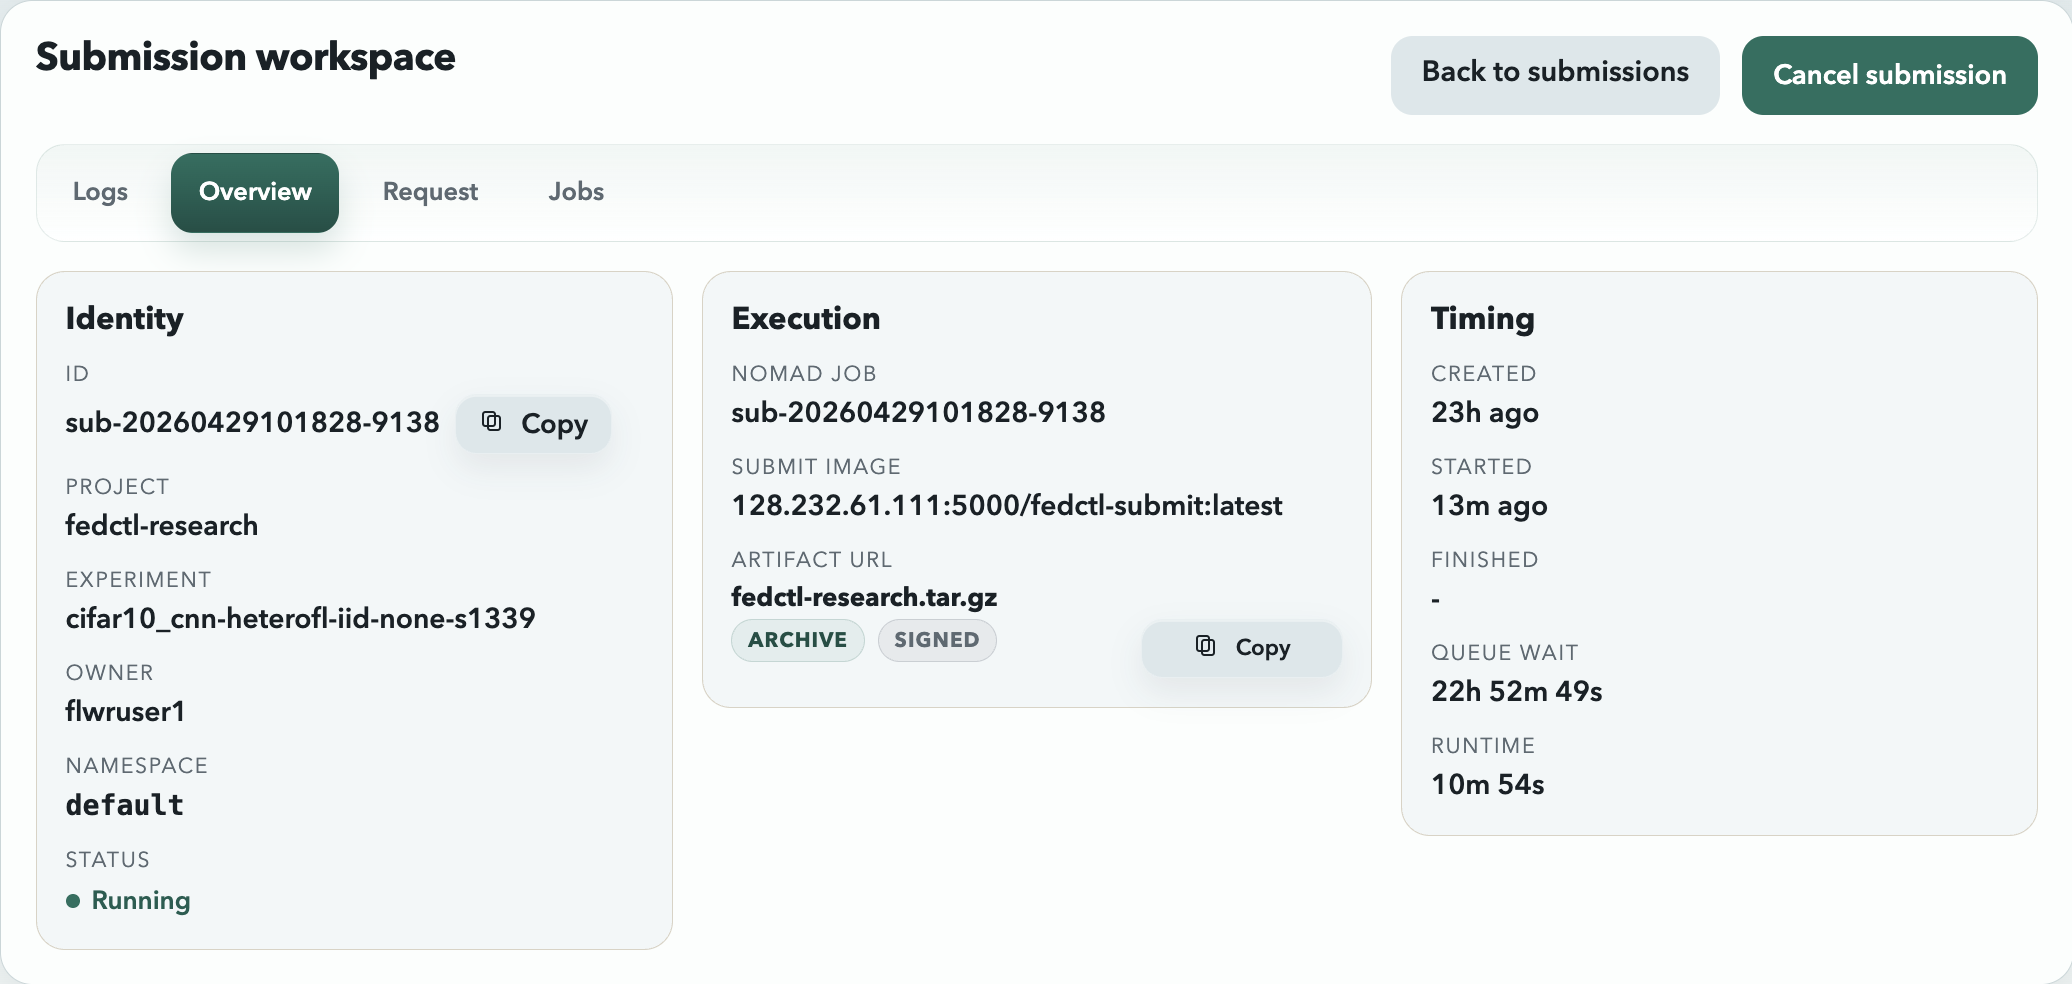
\includegraphics[width=\linewidth]{figures/detail_overview.png}
\caption{Run state and artefacts.}
\label{fig:submit_service_overview}
\end{subfigure}
\hfill
\begin{subfigure}[t]{0.48\textwidth}
\vspace{0pt}
\centering
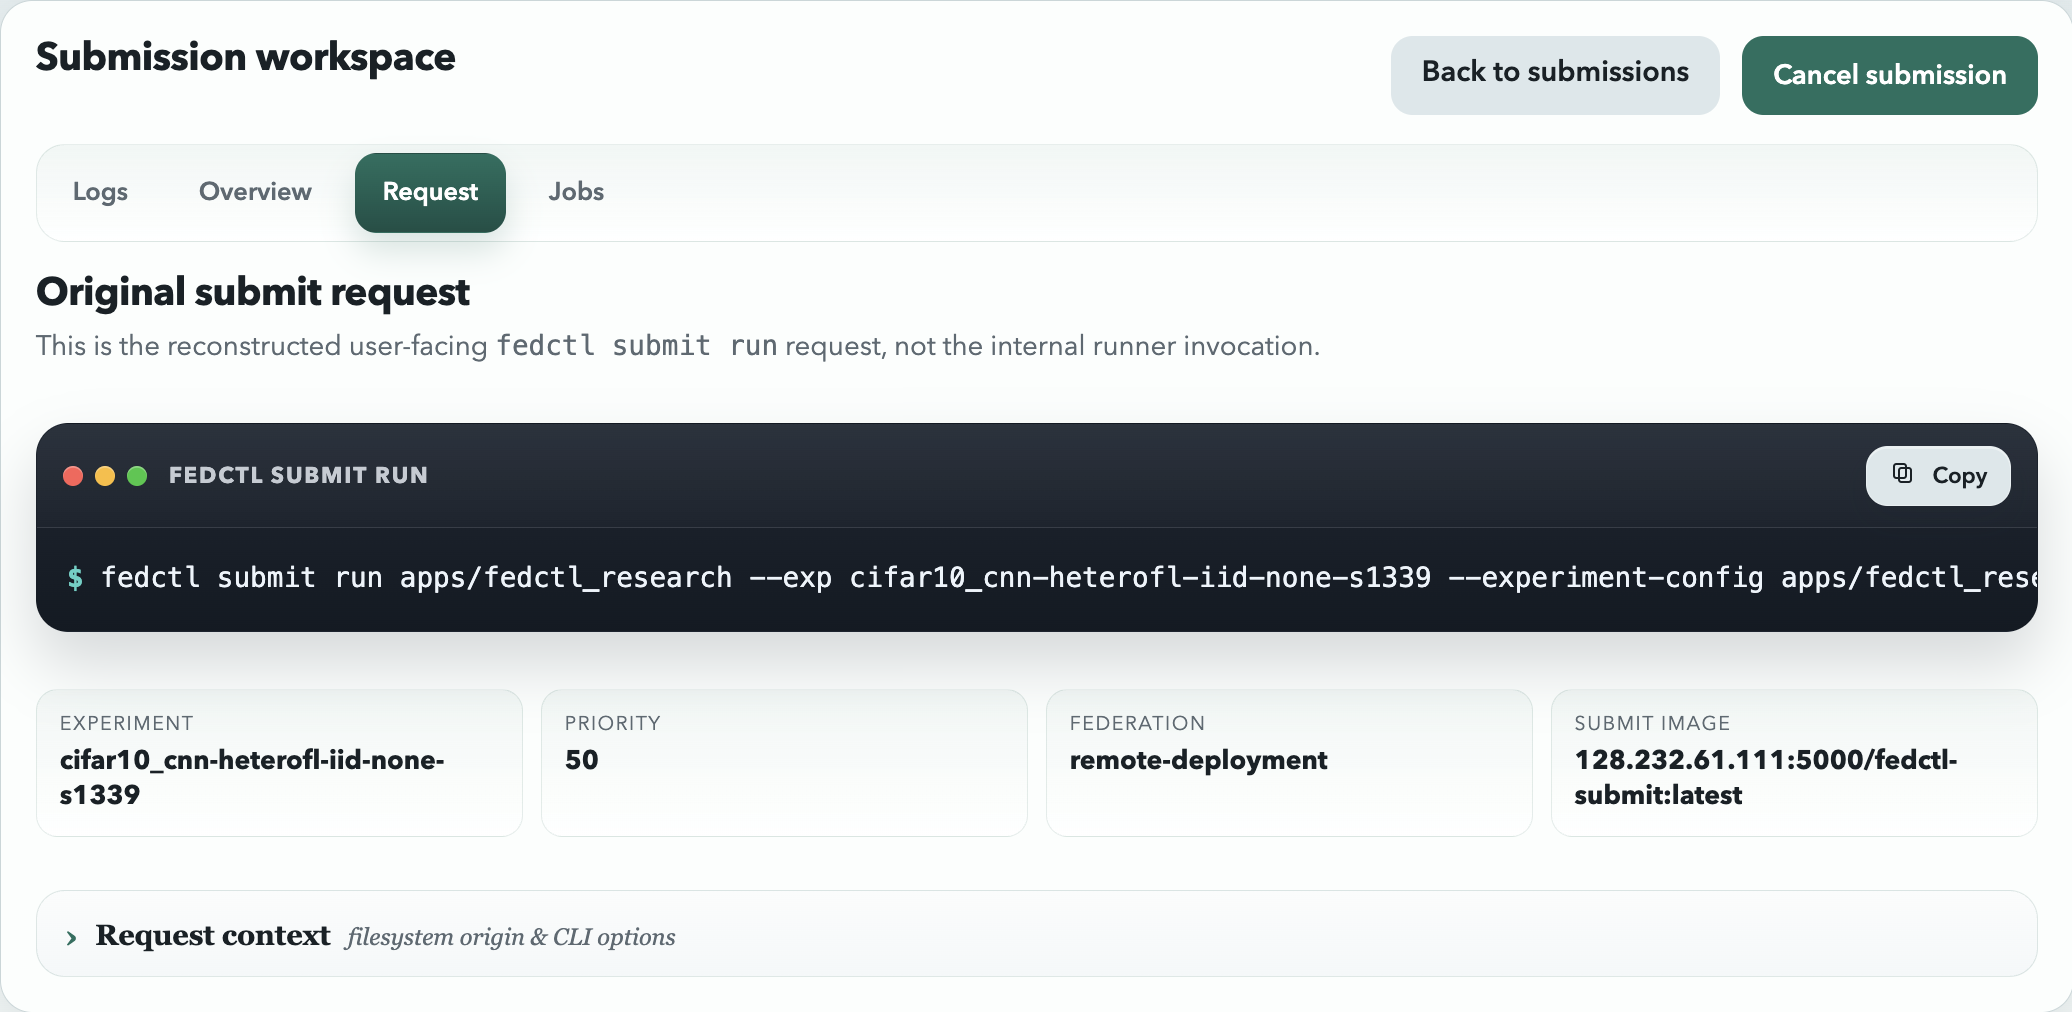
\includegraphics[width=\linewidth]{figures/detail_request.png}
\caption{Reconstructed request.}
\label{fig:submit_service_request}
\end{subfigure}
\par\vspace{0.6em}
\begin{subfigure}[t]{0.48\textwidth}
\vspace{0pt}
\centering
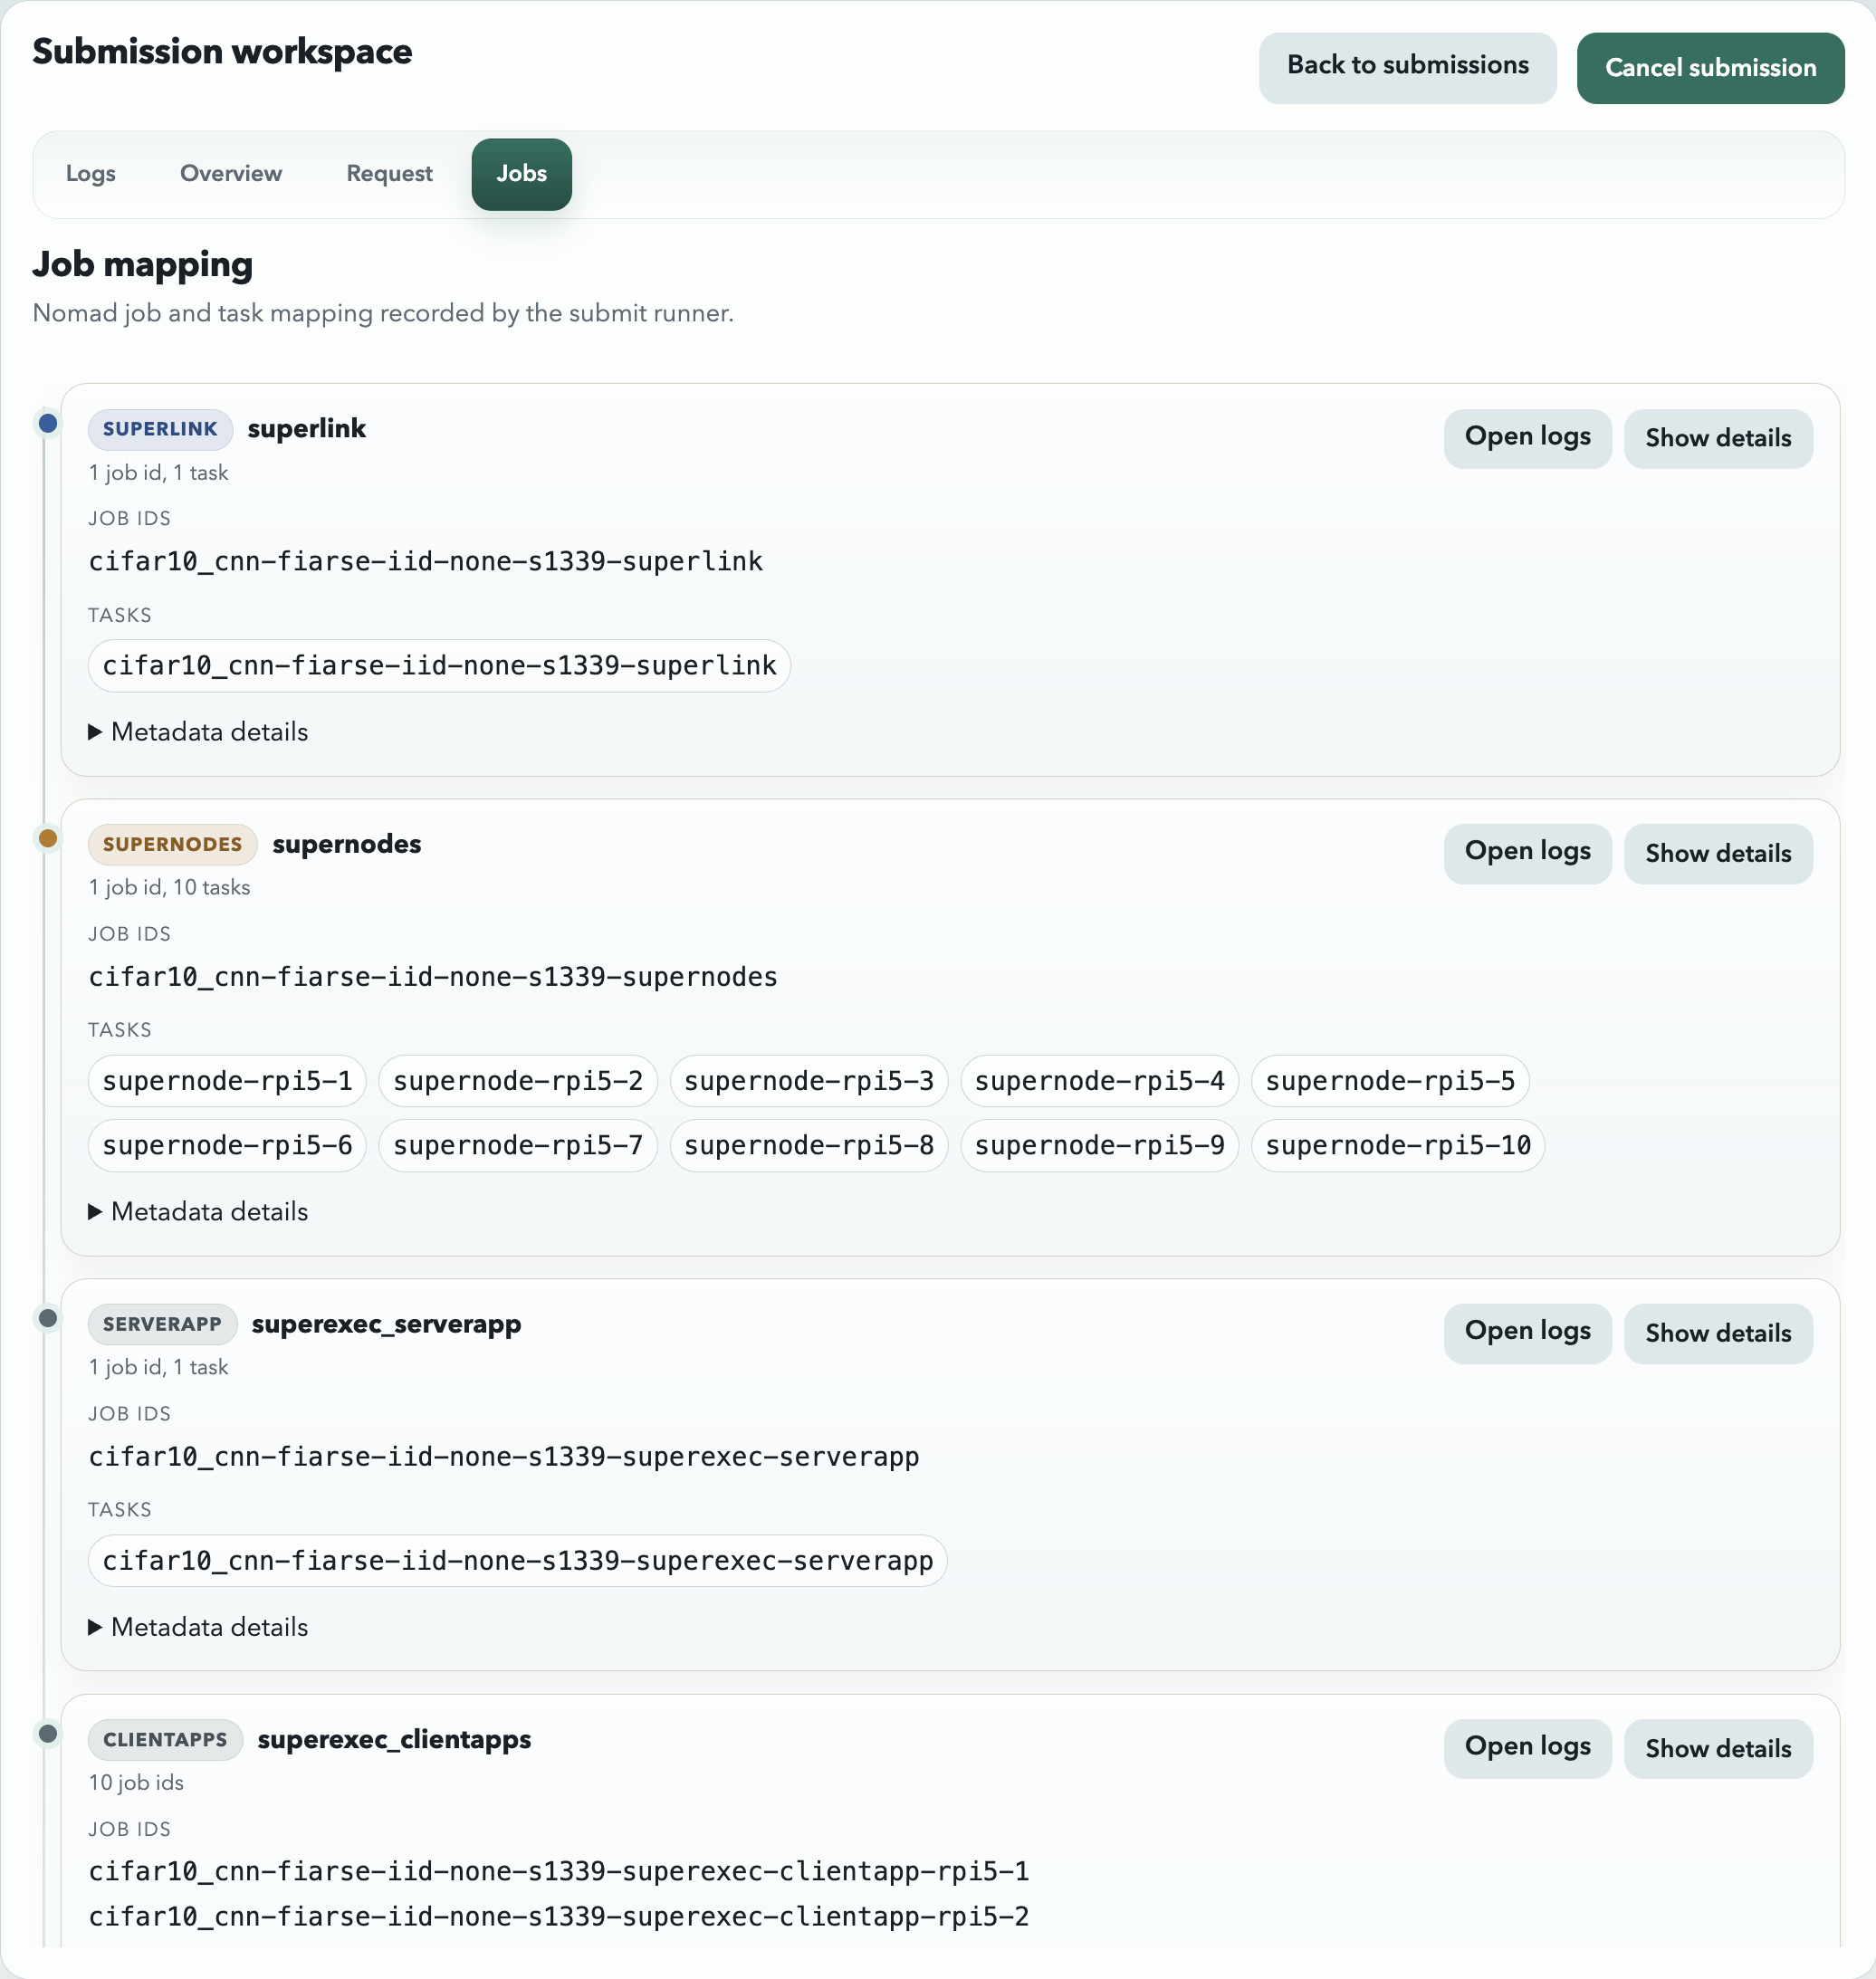
\includegraphics[width=\linewidth]{figures/detail_jobs.png}
\caption{Nomad role mapping.}
\label{fig:submit_service_jobs}
\end{subfigure}
\hfill
\begin{subfigure}[t]{0.48\textwidth}
\vspace{0pt}
\centering
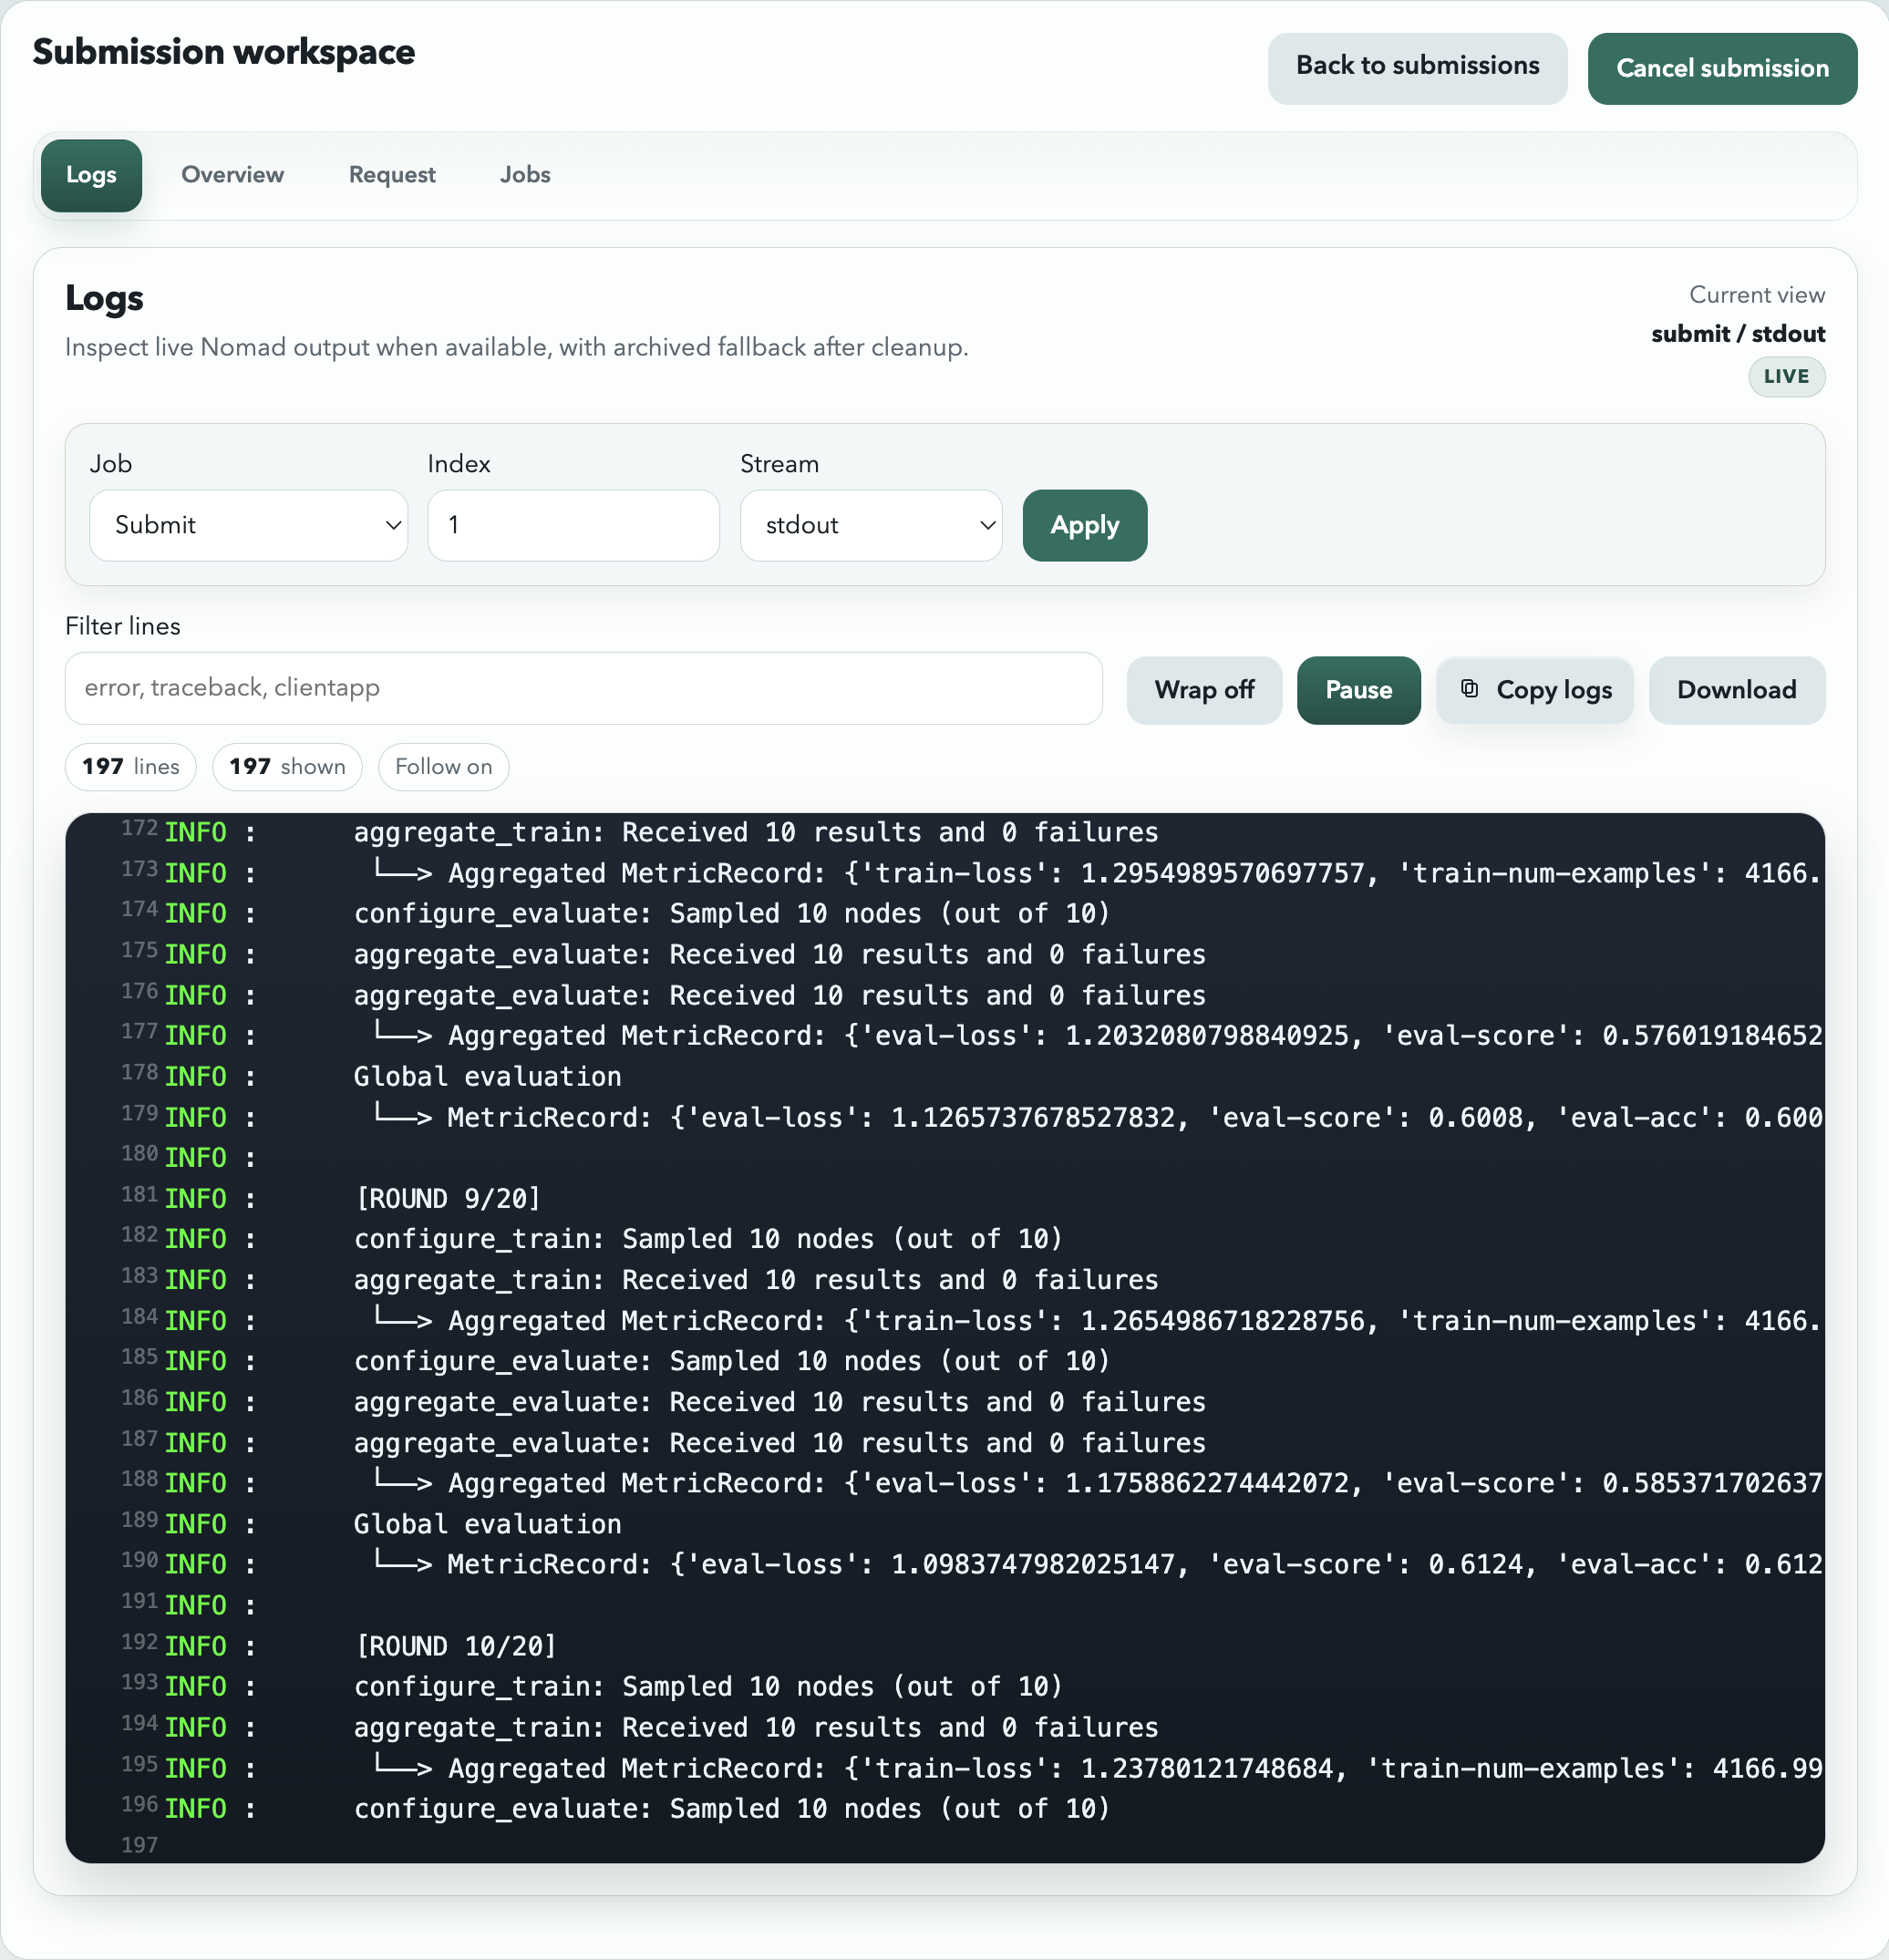
\includegraphics[width=\linewidth]{figures/detail_log.png}
\caption{Role logs.}
\label{fig:submit_service_logs}
\end{subfigure}
\caption{\textbf{Submit-service run-detail workspace.} The browser view keeps the state needed to reproduce, inspect, and debug a submitted run.}
\label{fig:submit_service_run_detail}
\end{figure}
